 \documentclass[12pt]{article}
\usepackage[a4paper, margin=.30in]{geometry}

\usepackage{array}
\usepackage{graphicx, subfig, wrapfig, fancyhdr, lastpage,makecell }
\newcommand\headerMe[2]{\noindent{}#1\hfill#2}
\usepackage[mathscr]{euscript}



\pagestyle{fancy}
\fancyhf{}

\rfoot{\em{Page \thepage \hspace{1pt} / \pageref{LastPage}}}
\begin{document}

\headerMe{Royaume du Maroc}{année scolaire \emph{2022-2023}}\\
\headerMe{Ministère de l'Éducation nationale, }{  Professeur :\emph{Zakaria Haouzan}}\\
\headerMe{du Préscolaire et des Sports}{Établissement : \emph{Lycée SKHOR qualifiant}}\\

\begin{center}

    \vspace{-1.5cm}
Devoir  N°3 - S1 \\
   Filière Tronc Commun Scientifique\\
Durée 2h00
\\
\hrulefill
\Large{Chimie 8pts - 48min}
\hrulefill\\

    \emph{Les deux parties sont indépendantes}
\end{center}
%end Headerss------------------------
 
    \vspace{-1.2cm}
    
\section*{Partie 1 :Géométrie de quelques molécules  \dotfill (5pts)}
%\begin{wrapfigure}[5]{r}{0.36\textwidth}
    %\vspace{-1.8cm}
    %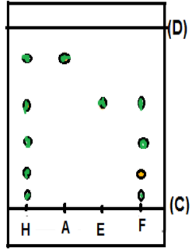
\includegraphics[width=0.36\textwidth]{./img/CCM.png}
%\end{wrapfigure}

On considère la molécule suivante de Chlorométhane $CH_3Cl$

\begin{enumerate}

\item Donner la structure électronique de carbone $C (Z=6)$, d’hydrogène $H (Z=1)$, et de chlore $Cl (Z=17)$ \dotfill(1pt)
\item  Donner le nombre $n_t$ des électrons de la couche externe de chaque atome \dotfill(1pt)
\item  Déterminer parmi ces atomes, les atomes qui obéissent à la règle du duet, et les atomes qui obéissent
à la règle de l’octet\dotfill(1pt)

\item   Déterminer le nombre de doublets liants $n_l$ et non liants $n_{nl}$ pour chaque atome. \dotfill(1pts)

\item  Représenter cette molécule selon le modèle de Lewis et déduire sa représentation de Cram \dotfill(1pt)

\end{enumerate}

\section*{Partie 2 :Classification périodique des éléments chimiques \dotfill (3pts) }
La couche électronique externe d'un atome est la couche (M). Elle comporte 1 électron. 
\begin{enumerate}
    \item Donner la structure électronique de cet atome.\dotfill(0.25pt)

    \item Dans quelle période et quel groupe de la classification périodique appartient l'élément chimique correspondant ?\dotfill(1pt)
    \item Donner son numéro atomique et l'identifier.\dotfill(1pts)
    \item Quel ion monoatomique est susceptible de se former à partir de cet atome ? \dotfill(0.25pt)
 \item Nommer la famille à laquelle cet élément chimique appartient. Citer deux éléments appartenant à la
     même famille.  \dotfill(0.5pt)
\end{enumerate}


%__________________Chimie ______________________-
%%%%%%%+_+_+_+_+_+_+_+_+_Partie1

%_____________________________________PHYSIque Partie 22222____________________________________________________________________________
\begin{center}
    %\vspace{2cm}
\hrulefill
\Large{Physique 12pts - 76min}
\hrulefill\\
    \emph{Les  parties sont indépendantes}
\end{center}

%\vspace{-1cm}
%end Headerss------------------------
\section*{Partie 1 :Relation entre la tension du ressort et son allongement \dotfill{(2pts)}}

\begin{wrapfigure}[2]{r}{0.38\textwidth}
	\vspace{-2.3cm}
 \begin{center}
	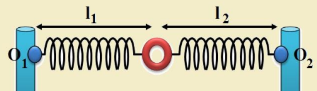
\includegraphics[width=0.38\textwidth]{./img/img00.png}
\end{center}
\end{wrapfigure}


On dispose de 2 ressorts. Le ressort $(R_1)$ a une longueur à
vide ${l_0}_1 = 10 cm$ et s’allonge de $1cm$ pour une force
appliquée de 1N. Le ressort $(R_2)$ a une longueur à vide
${l_0}_2=15cm$ et s’allonge de $3cm$ pour une force appliquée de 1N.

On les réunit à un anneau de poids et de dimensions
négligeables. Les deux autres extrémités des ressorts sont
fixées à deux crochets distants de $O_1O_2=30cm$. Soient $l_1$ et $l_2$ les longueurs respectives des ressorts $(R_1)$
et $(R_2)$.

\textbf{1.} Calculer la longueur de chaque ressort $l_1$ et $l_2$.\dotfill(1pt)

\textbf{2.} Calculer les intensités des forces de tension $F_1$ et $F_2$ des ressorts.\dotfill(1pt)


 \section*{Partie 2 :la poussée d'Archimède exercée sur un pavé \dotfill(5 pts)}
Un pavé flotte à la surface de l’eau. Ses dimensions sont : $h = 20 cm$ ,  $L = 60 cm$ ,  $l = 20 cm$.

\begin{wrapfigure}{r}{0.38\textwidth}
	\vspace{-5.3cm}

	
 \begin{center}
	 \hspace{-3cm}	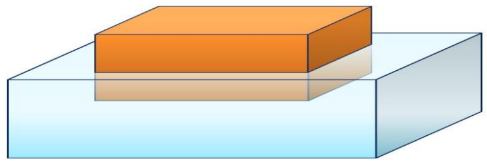
\includegraphics[width=0.38\textwidth]{./img/img01.png}
\end{center}
\end{wrapfigure}
\begin{enumerate}
	\item  Le pavé émerge sur une hauteur de $h' = 3 cm$. Calculer le volume V' de la partie immergée.\dotfill{0,5pts}

	\item  Calculer la masse $m'_{dep}$ d’eau déplacée.\dotfill{0,5pts}
	\item  Calculer le poids $P'_{dep}$ d’eau déplacé.\dotfill{0,5pts}
	\item  déduire la valeur du poids P du pavé.\dotfill{0,5pts}
	\item  Calculer la masse m du pavé.\dotfill{1pt}
	\item  Calculer le volume V du pavé.\dotfill{1pt}
	\item  Préciser le matériau constituant ce pavé.\dotfill{1pt}
\end{enumerate}

\textbf{Donnée: } La masse volumique d'eau: $\rho_{eau} = 1000 kg/m^3$ , L'intensité de pesanteur: $g = 10N/kg$.

\begin{center}
\begin{tabular}{ |c| c| c| c|c|c| }
	\hline
	\textbf{Matériau}                   & Polystyrène & Bois &glace &Aluminium&Fer\\\hline 
	\textbf{Masse volumique} $(kg/m^3)$ & 11 & 850 &920 &2700& 8000\\\hline
\end{tabular}
\end{center}

\section*{Partie 3 : la valeur de la poussée d'Archimède à l'aide d'un ressort \dotfill(5 pts)}

% \begin{center}
	%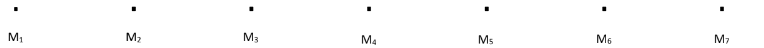
\includegraphics[width=0.8\textwidth]{./img/ex2.png}
%\end{center}

	%\vspace{-5.3cm}	

Un corps de masse m = 240 g est accroché à un dynamomètre à ressort.
L’allongement du ressort est 4 cm lorsque le corps est dans l’air.




\begin{enumerate}
	\item Calculer le poids du corps.\dotfill{0,5pts}
	\item  Que représente l’indication donnée par le dynamomètre. Quelle est sa
valeur ? Justifier.\dotfill{0,5pts}
\item  Déduire la valeur de la constante de raideur K du ressort.\dotfill{0,5pts}

	\vspace{-0.5cm}
 \begin{center}	
	 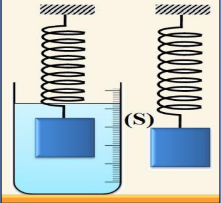
\includegraphics[width=0.2\textwidth]{./img/img02.png}
\end{center}
	\vspace{-0.5cm}

	\hspace{-1cm}Lorsqu’on plonge le corps entièrement dans un liquide contenu dans un
vase gradué, l’allongement du ressort devient $3,8 cm$ et le niveau du liquide
monte de $20cm^3$.

	\item	Calculer la masse volumique du corps.\dotfill{0,5pts}
	\item Calculer la tension du ressort quand le corps est dans le liquide. Quelle est, dans ce cas l’indication
du dynamomètre ? Que représente cette indication ?\dotfill{1pt}
\item  Déduire la valeur de la poussée d'Archimède exercée par le liquide sur le corps.\dotfill{1pt}
\item Calculer la masse volumique $\rho_L$ du liquide.\dotfill{1pt}
\end{enumerate}
\textbf{Donnée: }L'intensité de pesanteur: g = 10N/kg.

   %\vspace{5cm}
\begin{center}
\hrulefill
    \emph{Prove yourself to yourself not others.}
\hrulefill\\
\end{center}
%\begin{wrapfigure}[4]{r}{0.36\textwidth}
	%\vspace{-0.8cm}
	%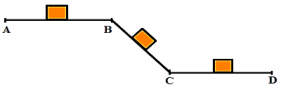
\includegraphics[width=0.36\textwidth]{./img/last.png}
%\end{wrapfigure}
\end{document}
